\subsubsection{Smart contract}
\label{sec:smart-contract}

The smart contracts in Ethereum are part of the application layer. They can be
referred to as implementing the business logic of the applications that runs on
the Ethereum system. A smart contract implements functions and has a state which
can be persisted and accessed in a subsequent execution. They can implement
\emph{almost} any function which can be implemented in any Turing-complete
machine. The difference is due to the gas needed for a transaction to be
executed: since the gas cannot be infinite, there will be always an upper bound
on the possible total amount of computation~\cite{wood2018ethereum}.

Usually, a smart contract is written in a high-level language, e.g. Solidity
(\autoref{sec:solidity}) or
Vyper\footnote{\url{https://github.com/ethereum/vyper}}, then compiled in EVM
bytecode. The contracts communicate with each other and with external actors
through their Application Binary Interface (ABI) represented in
\autoref{fig:abi}. This interface serves as a declaration of the functions
implemented by the contract and their arguments, thus another actor can trigger
the execution of it and get its result. The execution takes place in the EVM.

\begin{figure}
	\begin{center}
		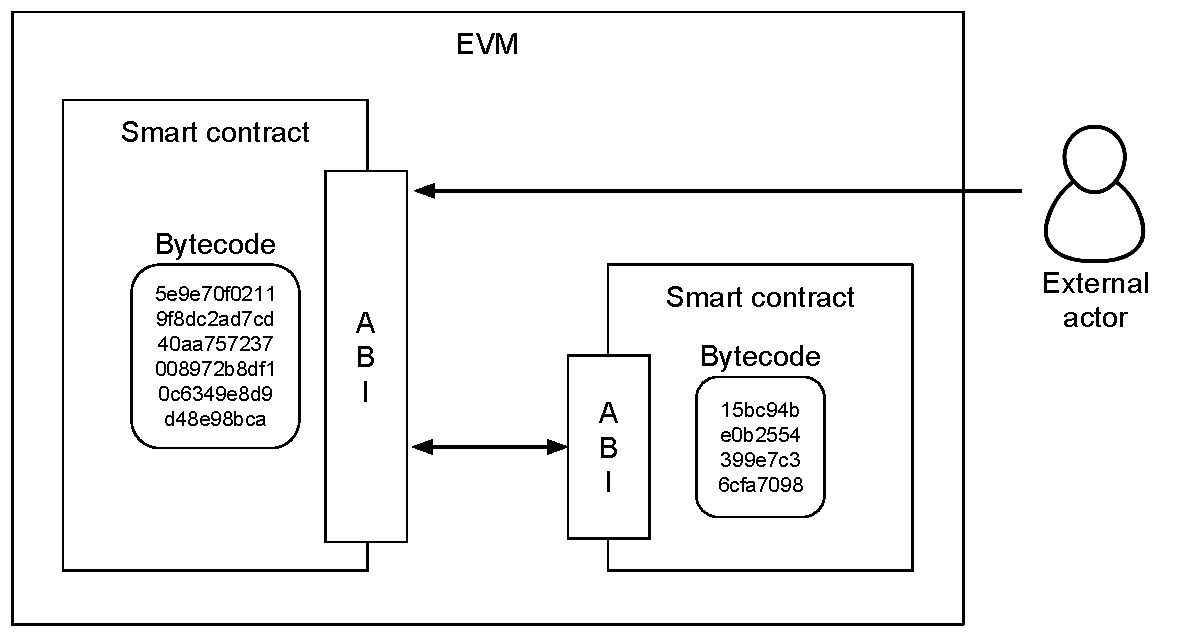
\includegraphics[width=0.7\textwidth]{./res/img/abi.pdf}
	\end{center}
	\caption{ABI representation.}
	\label{fig:abi}
\end{figure}

Although there is a common agreement on the ABI format~\cite{bib:solidity-docs},
this abstraction is not part of the core Ethereum protocol meaning that anyone
can define and expose its own ABI, but the caller have to comply to the format
used by the callee.
